\documentclass[11pt]{report}

\special{papersize=8.5in,11in}

\topmargin -0.5in \oddsidemargin 0.00in \evensidemargin 0.00in
\textwidth 6.75in \textheight 9.0in \headheight 0.25in \headsep
0.25in \footskip 0.5in \hoffset 0in \marginparpush 0.0in
\marginparwidth 0.0in \marginparsep 0.2in

\setcounter{page}{1}

\newcommand{\D}{\displaystyle}\newcommand{\T}{\textstyle}
\newcommand{\e}{{\mathrm{exp}}}
\newcommand{\dd}{{\mathrm d}}
\newcommand{\comment}[1]{}
\newcommand{\mb}{\mathbf}
\reversemarginpar

\usepackage[final]{graphicx}
\usepackage{fancyhdr}
%\graphicspath{{Papers/}}
\usepackage{amsthm,amssymb,amsmath}
\usepackage{cite}
\usepackage{geometry}
\usepackage{amsmath}
\usepackage{booktabs}
\usepackage{color}
\usepackage{setspace}
\usepackage{subfigure}
\usepackage{url}
%\usepackage[top=2.5cm, bottom=2.5cm, right=3.5cm, left=3.5cm]{geometry}
\geometry{a4paper,scale=0.8}
\setcounter{secnumdepth}{3}

\title{Research Progress Report}

\author{Botao Zhu}

\begin{document}
	
	\maketitle
	\lhead{\sf Research Progress Report-6th} \chead{} \rhead{\sf Botao Zhu}
	\lfoot{CTRG, University of Saskatchewan} \cfoot{} \rfoot{Page \thepage}
	\renewcommand{\footrulewidth}{1.0pt}
	\renewcommand{\headrulewidth}{2.0pt}
	\renewcommand{\arraystretch}{1.3}
	\pagestyle{fancy}
	
	\renewcommand{\thesection}{\arabic{section}}
	
	\section{Reading and Research Activities}
	
	\subsection{Reading Summary}
	
	
	
	
	\subsubsection{LEACH}
	
	\noindent LEACH \cite{926982} is the most representative clustering routing protocol, which has many advantages. Firstly, due to the application of time division multiple access (TDMA) in the communication between nodes, TDMA can avoid the collision problem of conventional nodes in the communication. In addition, each cluster is isolated from other clusters, so that nodes in different clusters can use the same frequency communication, which greatly improves the reuse rate of frequency band. LEACH protocol has two characteristics: data compression and clustering. The former helps to reduce energy consumption in wireless sensor networks, and the latter helps to expand wireless sensor networks. 
	
	\begin{itemize}
		\item Network Model of LEACH Protocol\\
		
		There are the following assumptions:\\
		(a) The base station node is fixed by power supply, which means the energy is sufficient.\\
		(b) The initial energy of each node is identical.\\
		(c) The location of each node is known and all nodes are static.\\
		(d) The residual energy of each nodes is known, and the loss of its own energy can be adjusted.\\
		
	\end{itemize}
	
	\begin{itemize}
		\item Energy Model of LEACH Protocol\\
		
		Because the main energy consumption of the protocol is only for receiving and sending data, the first order radio model as the energy model is in line with the needs.\\
		
		\begin{figure}[h!]
			\centering
			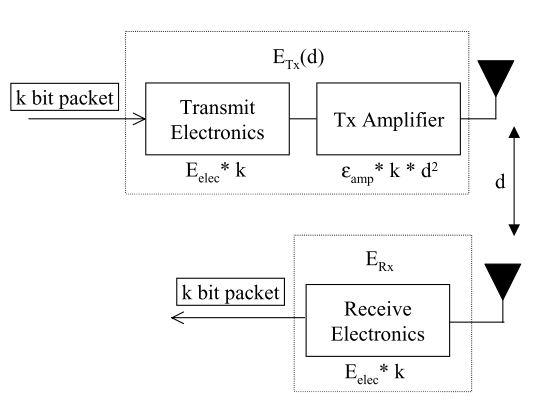
\includegraphics[width=0.6\linewidth]{firstordermodel.jpg}
			\caption{First order ratio model}
			\label{}
		\end{figure}
		As shown in the above figure, the energy consumption of nodes comes  from the sum of the energy consumption of signal transmitting, signal amplifying and receiving. The longer transmission distance each node has, the more the signal intensity will lose. Assuming the transmission distance is $d$, whenever the data of K bit is transmitted or received, the energy consumption formula of the transmitting is as follows\\
		\begin{equation}
		E_{send} = E_{TX\_elec}(k) + E_{TX\_amp}(k,d) = k\times E_{static} + k\times \sigma\times d^\beta
		\end{equation}
		the energy consumption formula of the receiving
		\begin{equation}
		E_{receive} = E_{RX\_elec}(k) = k \times E_{static}
		\end{equation}
		$E_{static}$ is the energy consumption of receiving and transmitting. Amplification multiples of signal amplifier is expressed as $\sigma$, $\beta$ is the route loss index. We need to choose the corresponding energy consumption model according to the length of transmission path for calculating the energy of data transmission. In the first-order radio energy consumption model, there are two kinds of distance $d$: self-space model and multi-path fading model. Free space model will be used at close range, and multi-path fading model will be used at long range. 
		\begin{equation}
		\left\{ \begin{array}{ll}
		\sigma_{fs}\times k \times d^2 & d \leq d_0 \\
		\sigma_{amp} \times k \times d^4 & d > d_0 \\
		\end{array} \right.
 		\end{equation}
		$\sigma_{fs}$ and $\sigma_{amp}$ represent the energy consumption parameters of amplifier of free space model and multi-path fading model respectively. $d_0$ is a threshold, which determines the model. 
		\cite{Chunyao2013AnEB} denotes:\\
		\begin{equation}
		d_0 = \sqrt{\frac{\sigma_{fs}}{\sigma_{amp}}}
		\end{equation}	
	\end{itemize}

	\begin{itemize}
		\item \textbf{Algorithm Implementation of LEACH Protocol}\\
		LEACH puts forward the concept of rounds, which divides the whole network into several rounds. In the set-up phase of each round, all nodes are divided into several clusters. Then in the steady-state phase of the protocol, the data will be transmitted to the base station according to certain rules. \\
		
		\textbf{Set-up phase}\\
		When the cluster has been established, it is necessary to select a node in each cluster to be the cluster head of the cluster. First, the nodes are randomly assigned a number between 0 and 1. Then the threshold of each node is calculated by the formula below. The node is selected as cluster head for the current round if the random value is less than the threshold, $T(n)$. Conversely, the node will become cluster member. 
		
		\begin{equation}
		T(n) = \frac{P}{1-P(r\text{mod}\frac{1}{p})}, \text{if} \, n \in G
		\end{equation}
		
		where P = the desired percentage of cluster heads, r = the current round, and G is the set of nodes that have not been cluster-heads in the past $\frac{1}{p}$ rounds. Each node will have a certain probability to become a cluster head. In the 0 round(r=0), the probability of each node becoming a cluster head is P. If the node is selected as cluster head in the 0 round, it is impossible for the node to become cluster head node in the next $\frac{1}{p}$ round. Because there are fewer nodes that are eligible to become cluster-heads, the probability that the remaining nodes are cluster-heads must be increased. \\
		When a node becomes a cluster head, it will broadcast a set of messages. Non-cluster-head nodes must remain in receiving state until they receive information from all cluster head nodes and join the corresponding cluster according to the intensity of broadcast information. When the cluster head node receives the 'join' message from the ordinary nodes in its cluster, it establishes plan table according to the TDMA. The plan table specifies when the cluster members can send data to the cluster head node. 
		\begin{figure}[h!]
			\centering
			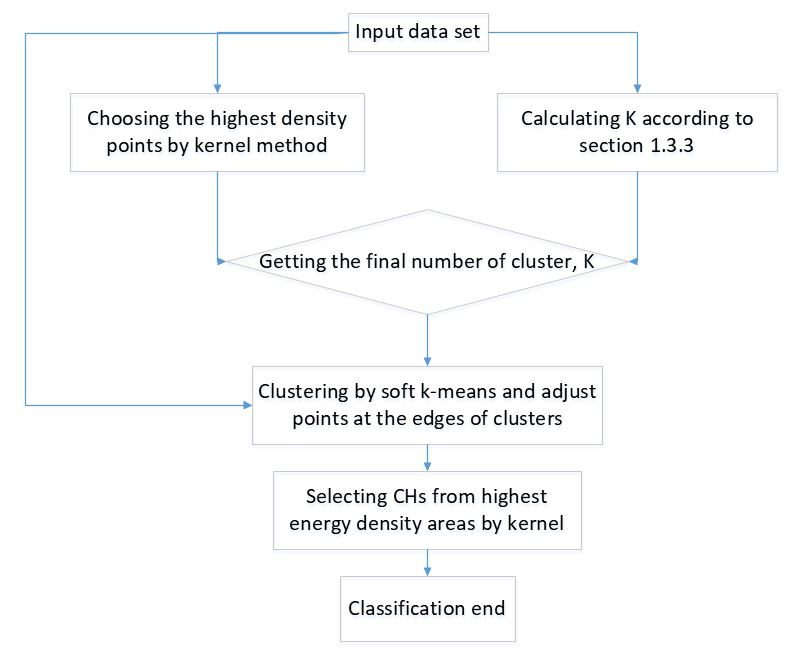
\includegraphics[width=0.6\linewidth]{flowchart.jpg}
			\caption{Cluster phase flowchart}
			\label{}
		\end{figure}
		
		  
		\textbf{Steady-state phase}\\
		When the cluster stage is completed, each node will have a corresponding cluster. Cluster members are scheduled by TDMA and transmit their data to cluster head node only with their own allocation time. Cluster members will remain dormant until their time slot arrives, which can reduce their energy consumption. At the same time, the cluster head node needs to keep its communication module open at any time, because it needs to receive data from cluster members constantly. 
		
		\begin{figure}[h!]
			\centering
			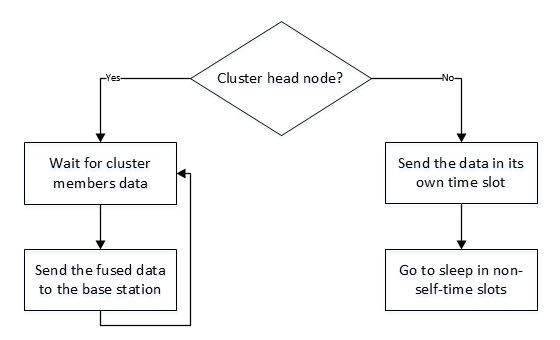
\includegraphics[width=0.6\linewidth]{phaseflowchart.jpg}
			\caption{Stable phase flowchart}
			\label{}
		\end{figure}
	\end{itemize}

	\begin{itemize}
		\item \textbf{Disadvantages of LEACH}\\
		
		1. It is possible to accelerate the death of cluster head nodes. The fact that a node may be selected as a cluster head in succession speeds up the death time of the cluster head node.\\
		
		2. There is no guarantee that cluster head nodes can cover the whole wireless sensor network. If the cluster head node is far from the member nodes, the energy consumption of data transmission between the two sides will increase, which will lead to abnormal death of the node. \\
		
		3. The distance between the base station and the cluster head is not considered. The cluster head node communicates directly with the base station by single hop, which causes  80\% of the energy loss comes from the distance transmission. 
	\end{itemize}
	

	\subsubsection{LEACH-C}
	
	\begin{itemize}
		\item \textbf{Set-up phase}\\
		LEACH-C\cite{1045297} is an improved version of LEACH, which uses a central control algorithm to form the cluster in the base station. During the set-up phase of every round, all nodes send their location by using a global positioning system and current energy to the base station. Determining optimal clusters is a NP-Hard problem, the base station needs to ensure the energy is evenly distributed in the whole network. The base station calculates the average node energy, and marks nodes as eligible cluster head nodes which have energy above average energy for the current round.  And then, \cite{104529777}the base station finds the best k nodes to be cluster heads by the simulated annealing algorithm, which attempts to minimize the amount of energy for the non-cluster head nodes to transmit their data to the cluster head, by minimizing the total sum of squared distances between all the non cluster head nodes and the closest cluster head. At each round, the next state $C'$, defined as a set of nodes, is depended on the current state $C$. To do this, the $x$ and $y$ coordinates of the nodes $c$ in $C$ were perturbed randomly for getting new  coordinates $x'$ and $y'$. The nodes closet to $(x',y')$ will become the new head nodes $c'$. Assuming $f(C)$ is the cost of current state and $f(C')$ is the cost of next state. The current state with probability: 
		\begin{equation}
		p_k = \left\{ \begin{array}{ll}
		e^{-\frac{f(C')-f(C)}{\alpha_k}},f(C) \leq f(C')\\
		1         \,                      ,f(C) > f(C')
		\end{array} \right.
		\end{equation}
		where $\alpha_k$ is the control parameter, 
		\begin{equation}
		\alpha_k = 1000e^{\frac{k}{20}}
		\end{equation}
		and
		\begin{equation}
		f(C) = \sum_{i=1}^{N}\text{min}\,d^2(i,c)
		\end{equation}
		$d(i,c)$ is the distance between node $i$ and node $c$.\\
		When the set-up phase is completed, the base station broadcasts a message contains the cluster head ID to all the nodes. If a node’s cluster head ID matches its own ID, the node is a cluster head; otherwise, the node determines its TDMA slot for data transmission and goes to sleep until it is time to transmit data.
	\end{itemize}
	
	\begin{itemize}
		\item \textbf{Steady-state phase}\\
		The steady-state phase of LEACH-C is identical to that of LEACH.
	\end{itemize}
	
	\begin{itemize}
		\item \textbf{Disadvantages of LEACH-C}\\   
		All nodes in the WSN must be within the communication range of BS, which greatly limits the size of WSN. The optimization results based on simulated annealing algorithm may have local optimum, so clustering may not reach global optimum. Also, simulated annealing algorithm needs a long running time, especially when the network scale is very large, which leads to more complex calculation and higher energy consumption, and greatly slows down the convergence speed. 
	\end{itemize}
	
	\subsubsection{E-LEACH}
	Energy-LEACH(E-LEACH) protocol \cite{4394931} is a kind of energy-based protocol. Cluster head nodes are elected on the basis of the maximum residual energy of nodes, not random selection like LEACH, which means nodes with less energy will not become cluster head nodes. In the cluster head election stage, instead of using probability $T(n)$, the residual energy of nodes is added to form a new threshold formula. In each round, nodes with more residual energy turn into cluster heads and send cluster head message to inform other nodes. The other nodes with less residual energy turn into common nodes and send information about joining cluster to a head. However, because all nodes need to send their residual energy information to the base station in order to select cluster head nodes in the base station, the energy consumption of the whole network is too fast. 
	\begin{figure}[h!]
		\centering
		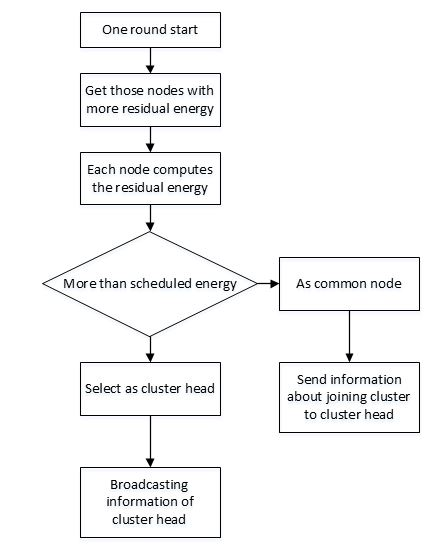
\includegraphics[width=0.5\linewidth]{eleachflowchart.jpg}
		\caption{E-LEACH flowchart}
		\label{}
	\end{figure}\\
	Fig. \ref {residualenergy} shows E-LEACH has the same residual energy as LEACH in the beginning, but E-LEACH has more residual energy than LEACH after a certain period of time.  
	\begin{figure}[h!]
		\centering
		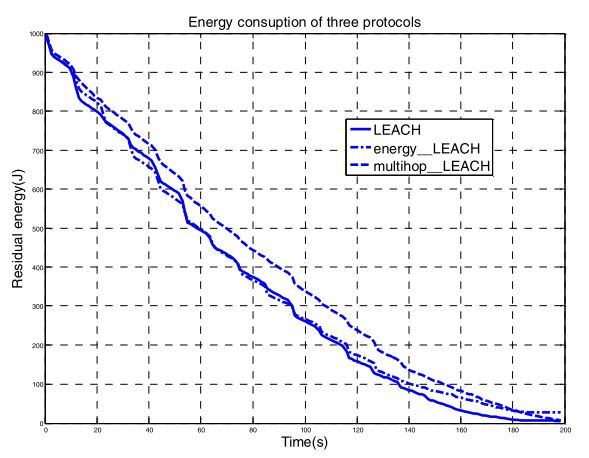
\includegraphics[width=0.5\linewidth]{eleach.jpg}
		\caption{Residual energy}
		\label{residualenergy}
	\end{figure}

	\subsubsection{M-LEACH}
	Instead of communicating directly with the base station, cluster head nodes in multihop-LEACH (M-LEACH)\cite{7342720} communicate with the nearest cluster head nodes  and transmit data through multiple hops, which reduces energy consumption of each node in wireless network and prolong the life of the network.  The disadvantage is that the protocol is complex and needs routing management. The cluster head nodes closer to the base station is not only responsible for the communication with the base station to transmit its own cluster data, but also responsible for forwarding the data of other clusters to the base station, which increases energy consumption of these nodes.
	
	
	
	\subsubsection{EEE-LEACH}
	The design idea of energy efficient extended LEACH (EEE-LEACH) \cite{6200608} is a two-layer cluster head transmission mechanism. Cluster and cluster head selection are the same as LEACH. Firstly, cluster heads are elected according to the threshold $T(n)$ of LEACH to form a set. Based on this set, the master cluster heads set is formed, which is responsible for sending the data from cluster head nodes to the base station. The cluster head nodes are responsible for data fusion and transmission within the cluster. The number of master cluster head nodes is less than the number of cluster head nodes, so the energy consumption of cluster node heads can be reduced by adding the master cluster head layer. 
	\begin{figure}[h!]
		\centering
		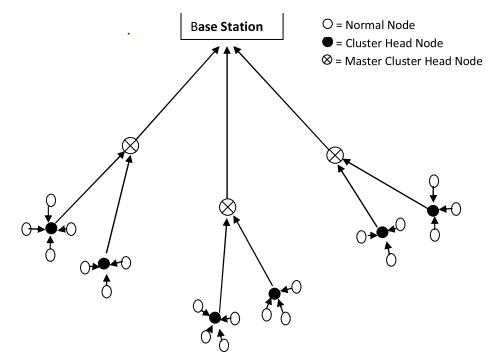
\includegraphics[width=0.5\linewidth]{eeeleach.jpg}
		\caption{Cluster organisation of EEE-LEACH}
		\label{}
	\end{figure}

    \begin{figure}[h!]
		\centering
		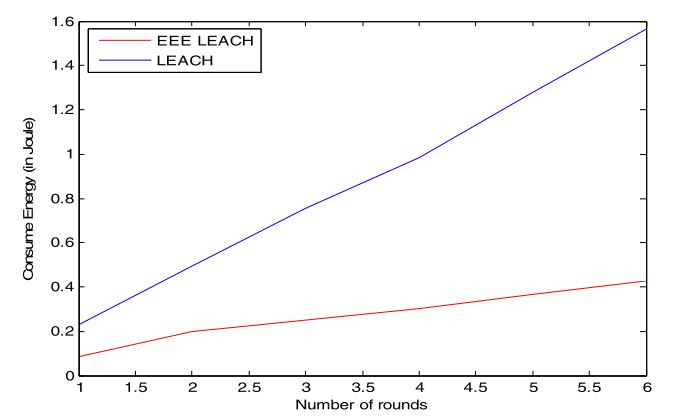
\includegraphics[width=0.5\linewidth]{eeeleach1.jpg}
		\caption{Energy Consumption of LEACH and EEE-LEACH}
		\label{eee1}
	\end{figure}
	Fig. \ref {eee1} shows the comparison between LEACH and EEE-LEACH in terms of energy consumption, EEE-LEACH is more energy efficient than LEACH. 

	
	\subsubsection{V-LEACH}
	In order to improve the network life, the vice cluster head LEACH (V-LEACH) was proposed \cite{6524310}. The process of vice cluster head selection on the basis of three factors: minimum distance, maximum residual energy and minimum energy. Normally, the cluster heads complete all the work, and the vice-cluster heads fall into dormancy, so as to reduce energy consumption as much as possible. As a cluster head will die, it will be replaced by its vice-cluster head. This protocol can avoid the sudden death of cluster head node and the sudden stop of data transmission, but the cluster head nodes of this protocol communicate with the base station in a single hop mode. 
	\begin{figure}[!h]
		\subfigure[Dead nodes in LEACH]{
			\begin{minipage}[h]{0.4\linewidth}
				\centering
				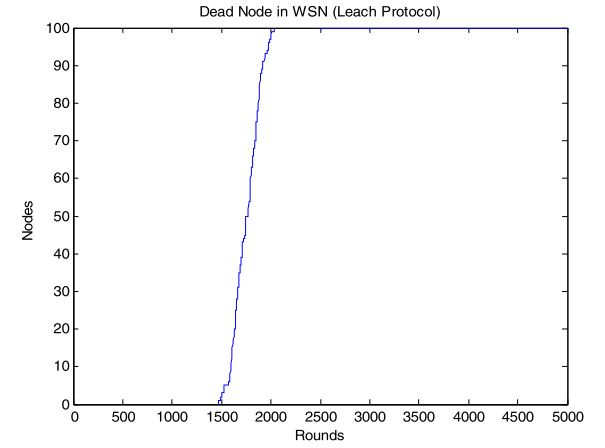
\includegraphics[width=3in]{vleach1.jpg}
				\label{}
			\end{minipage}
		}%
		\subfigure[Dead nodes in V-LEACH]{
			\begin{minipage}[h]{0.4\linewidth}
				\centering
				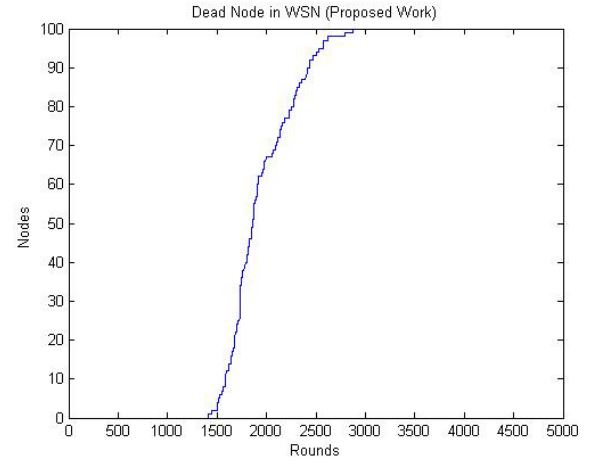
\includegraphics[width=3in]{vleach2.jpg}
				\label{}
			\end{minipage}
		}%
		\centering
		\caption{Dead node comparison}
	\end{figure}
	
	
	
	\section{Objectives for the Next 2 Weeks}
	\subsection{Reading} 
	Searching and reading papers of applied machine learning in LEACH.
	
	
	\section{Advisor's Comments}
	
	\bibliographystyle{IEEEtran}
	\bibliography{janbib}
	
\end{document}